% https://tex.stackexchange.com/questions/752322/macro-for-automating-marking-table-in-exam-class
\documentclass[12pt,addpoints,a4paper]{exam}
\usepackage{tikz}
\begin{document}
\begin{center}
    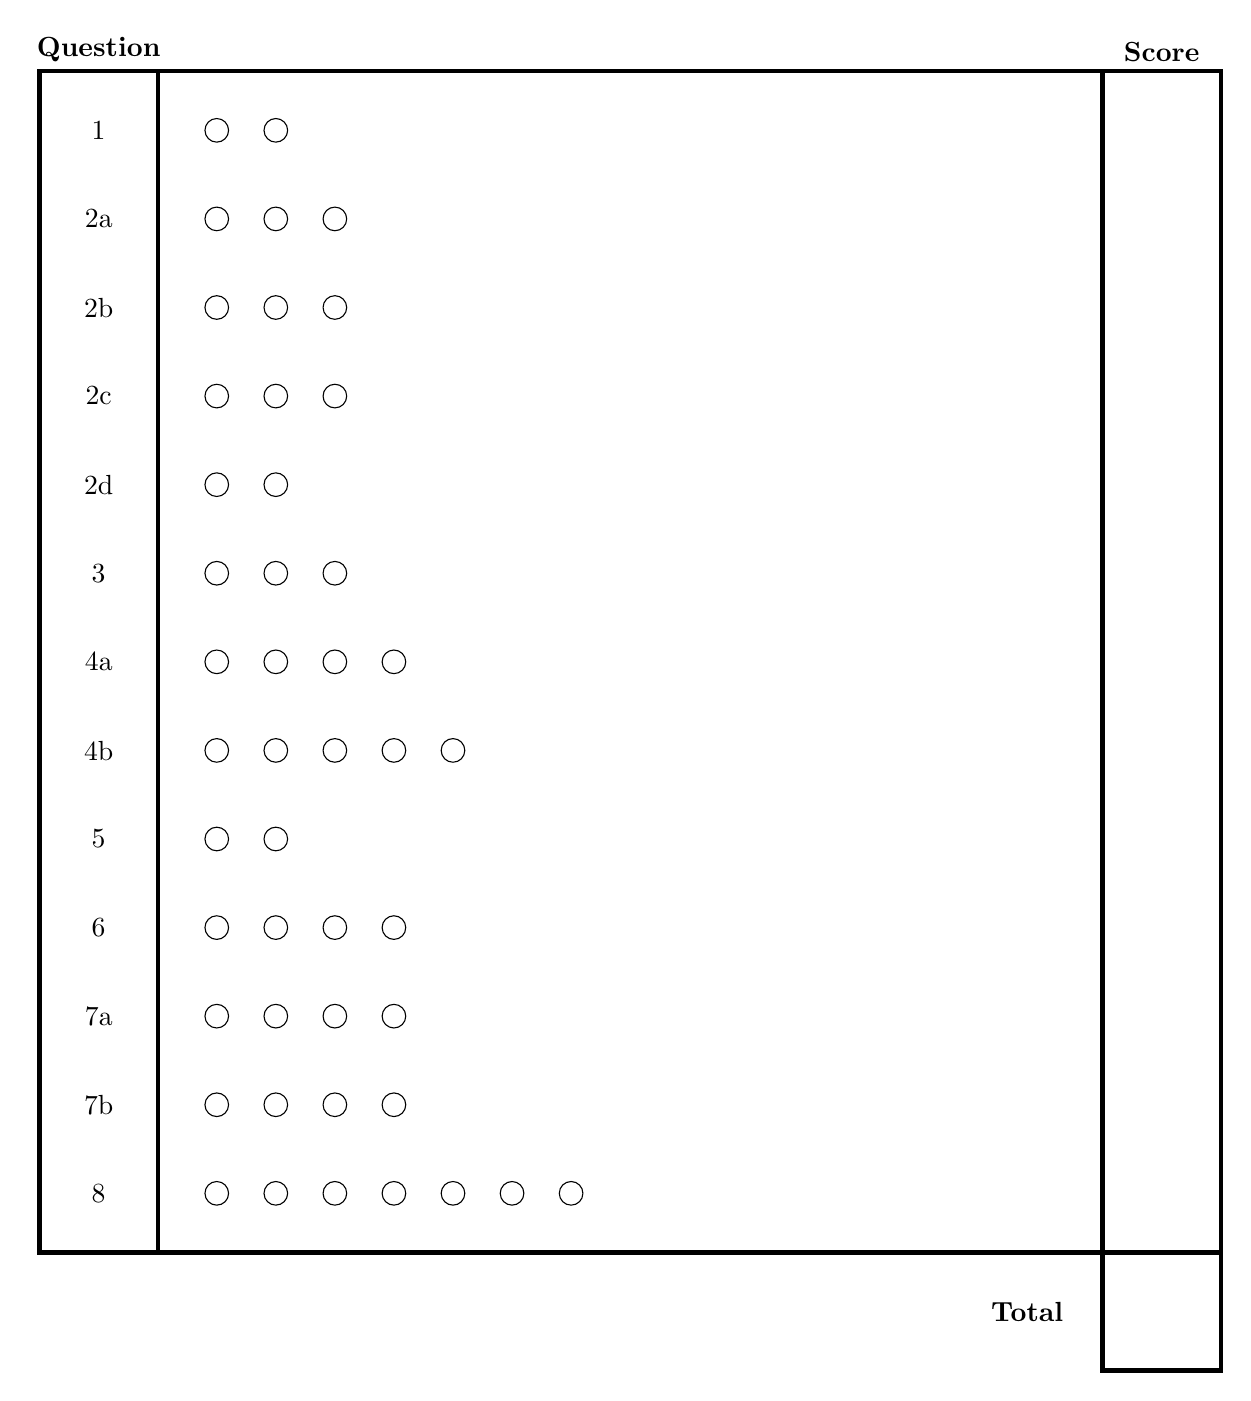
\begin{tikzpicture}[scale=.75]
    \draw[ultra thick]
        (-10,-1.5) rectangle (10,-21.5)
        (-8,-1.5) rectangle (8,-21.5)
        (8,-21.5) rectangle (10,-23.5);
    \path[nodes={font=\bfseries}]
        (7.5,-22.5) node[left]{Total}
        (9,-1.5) node[above]{\textbf{Score}}
        (-9,-1.5) node[above]{\textbf{Question}};
    \foreach \scorenum/\lab[%
            count=\n from 0,
            evaluate=\n as \mypos using -2.5-1.5*\n,
        ] in {%
        2/{$1$},
        3/{$2\mathrm{a}$},
        3/{$2\mathrm{b}$},
        3/{$2\mathrm{c}$},
        2/{$2\mathrm{d}$},
        3/{$3$},
        4/{$4\mathrm{a}$},
        5/{$4\mathrm{b}$},
        2/{$5$},
        4/{$6$},
        4/{$7\mathrm{a}$},
        4/{$7\mathrm{b}$},
        7/{$8$}%<- % is must
    }{
        \node at (-9,\mypos) {\lab};
        \foreach \x in {1,...,\scorenum}{%
            \draw (-8+\x,\mypos) circle[radius=0.2cm];
        }
    }
    \end{tikzpicture}
\end{center}
\end{document}